After a research and looking for suitable existing state modeling languages, it has been decided to create a new light-weight DSL for data representation based on run-time state migration requirements.
A DSL can be developed from scratch, or it can be a modification or a modified form of an existing domain-specific modeling language.

The Application State Modeling Language (ASML) is a DSL that defines any type of software application state.
The focus of this language is on modeling single types states of the run-time.

As mentioned in requirements \textbf{D1 State Specification}, this language supports run-time states that are migratable.
An application can have multiple states, and users can switch between them.
These states and their transition can be modeled in different ways (e.g., UML state machine diagram), but as we analyzed some applications in requirements (Chapter \ref{ch:requirements}), we deal with the data perspective of run-time states and have to access to the actual values and migrate them. Therefore, the run-time state’s actual data will be migrated not their transition. For example, Amazon States Language considers the state transition as some tasks that need to be done step by step.
Moreover, there is no need to include the transition between states in state specification as we assume we know in which state application is. 

Each model can cover only an individual state. The advantage of having an individual model for each state is improving interoperability, allowing different domain applications to share a specific part of them.
For example, an e-mail application may have a calendar that can migrate data with a mobile phone calendar application.
Also, there is no need to model the states which are not migratable. So, it reduces the time of modeling state and the amount models. 

Figure \ref{fig:asml-overview} shows an overview of Application State Modeling Language (see \fcircone). The specification of a type of state using the ASML is called an Application State Model (see \fcirctwo), which is discussed in subchapter 5.2. There are some applications support the run-time state migration and have common Application State Models (see \fcircthree). The  actual values of a state on run-time is Run-Time State, which is discussed in subchapter 5.3.

\FloatBarrier
\begin{figure}[H]
    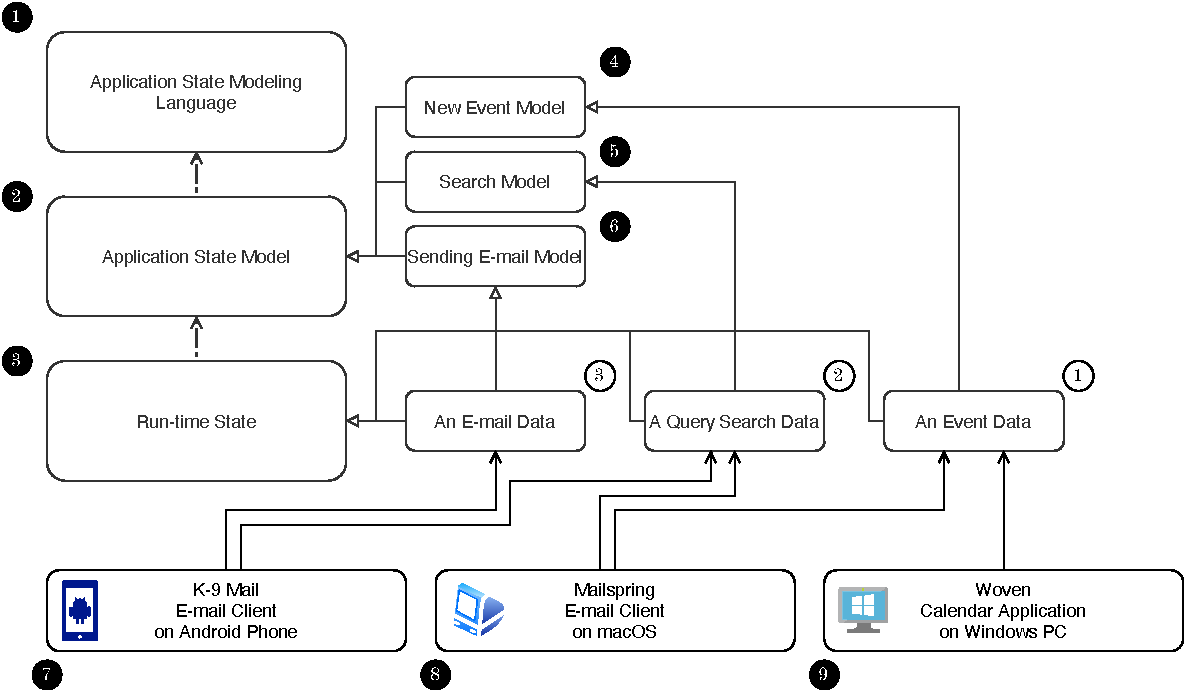
\includegraphics[scale=0.8]{../figures/asml-overview.pdf}
    \centering
    \caption{Overview of Application State Modeling Language}
    \label{fig:asml-overview}
\end{figure}
\FloatBarrier

Considering three states which are modeled as \textit{Sending E-mail Model}, \textit{Search Model} and \textit{New Event Model}. In this example, we have three applications which are K-9 Mail is an e-mail client on an Android phone, Mailspring is another e-mail client which also has calendar management on macOS, and Woven Calendar is a calendar application for Windows. K-9 Mail has two migratable run-time states, which are \textit{Sending E-mail} and \textit{Search}. Mailpsring has three migratable states, which are \textit{New Event}, \textit{Sending E-mail} and \textit{Search}. Waven has two migratable run-time states, which are \textit{New Event} and \textit{Search}. As Mailpsring and Waven have a mutual \textit{New Event} run-time state, they can share a common model: the \textit{New Event Model}. However, Mailspring has two other common run-time states which have common models with K9 Mail: the \textit{Sending E-mail Model} and \textit{Search Model}. So, Mailspring and Woven can migrate actual run-time data of the \textit{New Event} state. Furthermore, Mailspring and K-9 can migrate actual run-time data of the \textit{Sending E-mail} state and the \textit{Search} state. This shows the same model can be used for different applications. The figure will be further explained in detail in the relevant sections.

\subsection{Metamodel}
Figure \ref{fig:asml-meta-model} shows the metamodel of our DSL as an UML class diagram. An Application State Model can describe one state. Each state specified in the Application State Model has a unique name, a description and some keywords. The extra information of a state is the version and author that can be defined in Number and String. Each state can have multiple values. Each value also can have multiple values which consists of a unique name and a type which can be a primitive type like Array, Object, Boolean, File, Number, and String. Also, a value can have some constraints like format, regex pattern, required and etc.

\FloatBarrier
\begin{figure}
    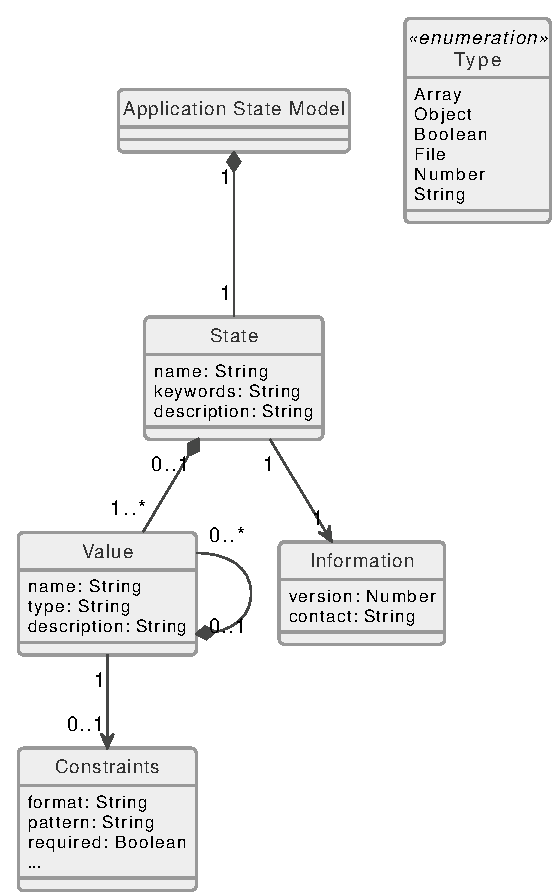
\includegraphics[scale=1]{../figures/asml-class-diagram.pdf}
    \centering
    \caption{UML Class Diagram of our DSL Metamodel}
    \label{fig:asml-meta-model}
\end{figure}
\FloatBarrier

\subsection{Language Stack}
There are many ways to define a DSL; it can be made from scratch (e.g., developing a language base on Xtext framework) or extended or restricted versions of other languages. The ASML is an extended version of JSON Schema. 

\subsection{Language Schema}
The ASML itself is a JSON Schema document based on JSON Schema Draft-07
\footnote{\href{https://json-schema.org/draft-07/json-schema-release-notes.html}{JSON Schema Draft-07 Release Notes}}
and is following the same logic and syntax. Table \ref{tab:asml-schema} shows the the schema of ASML with its most important properties in a condensed form. 
The full schema of ASML is available on its GitHub repository
\footnote{\href{https://github.com/asml-lang/asml/blob/master/schemas/schema.json}{https://github.com/asml-lang/}}.

\subsubsection{Mapping Metamodel to JSON Schema}
The metamodel of ASML (Fig. \ref{fig:asml-meta-model}) is mapped in JSON Schema. Therefore, each state should be defined in one JSON Schema document which is Application State Model. Each state should have a name, a description and keywords. Values of a state should be defined in \lstinline[basicstyle=\ttfamily]{properties} of JSON Schema, in which each value should be define as an object with a unique name as a key. The type of this value can be defined as a key-value pair inside value object, the key is “type” and its string value can be a primitive data type like number, string, boolean, and etc. Also, each value can have a description. The extra information like version and author’s contact are mapped to \lstinline[basicstyle=\ttfamily]{info} element. Moreover, each value can have some constrains like format, pattern and required that they can be defined inside value object. These constrains can be part of JSON Schema capabilities.

\FloatBarrier
\begin{table}[H]
\begin{tabularx}{\textwidth}{|l|X|X|r|}
\hline
Property             & Description                                                                              & Value                                                                                                                   \\\hline
title                & The name of the DSL.                                                                     & Application State Modeling Language                                                                                     \\\hline
description          & The description of the DSL.                                                              & A DSL for enabling run-time state migration between same-purpose applications of different vendors \\\hline
version              & The current version of the DSL, which can be used in for version checking for validating models. & 1.0.0                                                                                                                   \\\hline
properties           & Contains values which an Application State Model should have.                                       & \{"asml", "info", "properties", "required"\}                                                                            \\\hline
required             & Defining the required items which a model must have.                                     & {[}"asml", "info", "properties"{]}                                                                                      \\\hline
additionalProperties & The DSL is not allowing developers to add additional properties to models.               & false                                                                                                                   \\\hline
definitions          & Contains the definition of the DSL items and the basic JSON Schema specification.        & version, asml, info, contact, Schema

\\\hline
\end{tabularx}
\caption{ASML Schema}
\label{tab:asml-schema}
\end{table}
\FloatBarrier





